\documentclass[11pt,a4paper]{article}
\usepackage[T1]{fontenc}
\usepackage{lmodern,microtype,amsmath,amssymb,mathtools}
\input{ot1lmr.fd}
\DeclareFontShape{OT1}{lmr}{bx}{n}{<-> rm-lmbx10}{}
\DeclareFontShape{T1}{lmr}{bx}{n}{<-> ec-lmbx10}{}
\usepackage[margin=24mm,headheight=15pt]{geometry}
\usepackage{booktabs,longtable,tabularx,array,graphicx,xcolor,fancyhdr,enumitem}
\usepackage[colorlinks=true,linkcolor=blue!45!black,urlcolor=blue!45!black]{hyperref}
\hypersetup{pdftitle={What have we learned from joint SPX-VIX calibration?},pdfauthor={Project research synthesis},pdfsubject={Model mechanisms, experimental results and calibration tradeoffs}}
\definecolor{navy}{HTML}{17324D}
\definecolor{teal}{HTML}{168C8C}
\setlength{\emergencystretch}{2em}
\Urlmuskip=0mu plus 2mu
\expandafter\def\expandafter\UrlBreaks\expandafter{\UrlBreaks\do\A\do\B\do\C\do\D\do\E\do\F\do\G\do\H\do\I\do\J\do\K\do\L\do\M\do\N\do\O\do\P\do\Q\do\R\do\S\do\T\do\U\do\V\do\W\do\X\do\Y\do\Z\do\a\do\b\do\c\do\d\do\e\do\f\do\g\do\h\do\i\do\j\do\k\do\l\do\m\do\n\do\o\do\p\do\q\do\r\do\s\do\t\do\u\do\v\do\w\do\x\do\y\do\z}
\setlength{\parindent}{0pt}
\setlength{\parskip}{5.5pt}
\setlist{itemsep=2pt,topsep=3pt,leftmargin=1.5em}
\renewcommand{\arraystretch}{1.18}
\newcolumntype{Y}{>{\raggedright\arraybackslash}X}
\pagestyle{fancy}\fancyhf{}
\fancyhead[L]{\small\color{navy}SPX--VIX calibration: lessons from the experiments}
\fancyfoot[C]{\small\thepage}
\newcommand{\E}{\mathbb E^{\mathbb Q}}
\newcommand{\Var}{\operatorname{Var}}
\newcommand{\Cov}{\operatorname{Cov}}
\newcommand{\VIX}{\operatorname{VIX}}
\newcommand{\splus}{\operatorname{softplus}}
\newcommand{\src}[1]{\textcolor{teal}{\small[#1]}}
\newcommand{\lesson}[1]{\par\smallskip\noindent\colorbox{teal!9}{\parbox{\dimexpr\linewidth-2\fboxsep}{\textbf{What we learned.} #1}}\par\smallskip}
\title{\color{navy}\Huge What have we learned from\\[4pt]joint SPX--VIX calibration?}
\author{A mathematical and experimental synthesis of the project records}
\date{28 October 2026}
\begin{document}
\hypersetup{pageanchor=false}
\begin{titlepage}
\maketitle\thispagestyle{empty}
\vspace{8mm}
{\large An undergraduate-level guide to readouts, stochastic volatility response, stress timescales, leverage and calibration tradeoffs.}
\vspace{9mm}
\lesson{We have found useful mechanisms and substantial partial improvements, but no satisfactorily established double calibration. Two-speed stress greatly improves the tested VIX fit. Negative stock--stress dependence substantially improves SPX skew while preserving VIX. Further asymmetry and adaptive correlation experiments have not closed the remaining gap.}
\vspace{5mm}
This report separates mathematical identities, observed calibration results, numerical limitations and untested ideas. It covers the documented model changes and groups the many estimator experiments by what they taught us. It is a synthesis of existing experiments, not a new calibration run.

\textbf{Evidence cutoff.} The latest completed record reviewed is the 28 October future-integrated-variance leverage experiment. Earlier notes sometimes describe later-completed experiments as proposals; this report uses the later results.

\textbf{Market scope.} The pricing research uses the 19 February 2026 snapshot. The current retained maturities are seven SPX dates and four VIX dates. Current scores are in sample with respect to market observations. New simulation seeds check numerical stability, not a new market date.

\vfill
\textbf{Reading guide.} Read Sections 1--3 for the framework, Sections 4--11 for the model experiments, and Sections 12--14 for numerical lessons, the experiment map and the remaining research questions. Source identifiers in brackets refer to the local records listed in the appendix.
\end{titlepage}
\hypersetup{pageanchor=true}
\pagenumbering{roman}
\tableofcontents\clearpage
\pagenumbering{arabic}

\section{The main findings before the details}

The most useful way to organize the work is around four different controls:
\begin{enumerate}
\item \textbf{The forward-variance curve gives the average variance budget.} It controls how much variance is available at each future time. A clever readout cannot compensate for an insufficient budget when option prices imply a larger necessary second moment.
\item \textbf{The readout distributes that budget across states.} Caps, shifted quadratics, products and additive mixtures determine whether variance comes from ordinary states, rare stress states, or both. Normalization matters: increasing an unnormalized response does not increase every normalized state.
\item \textbf{Persistence controls how long shocks survive.} A brief burst and a persistent episode can have similar instantaneous variance but very different effects on 30-day average variance and multi-month option smiles.
\item \textbf{Stock--factor dependence controls which equity moves accompany high variance.} Negative dependence can strengthen SPX downside skew without changing VIX, provided the complete variance-factor law is preserved.
\end{enumerate}

The strongest VIX-only result is the shared two-speed additive stress model: checking option loss fell from 1.7256 to 0.0501, and prices inside bid--ask rose from 83 to 153 of 217. This is a large improvement, but some forward errors remain and the checking sample was partly reused. \src{R13}

The clearest SPX improvement that protects VIX is the mixed negative Brownian rotation: checking SPX interval loss fell by 50.9\%, and implied-volatility mean absolute error fell from 4.493 to 3.199 percentage points. Yet only 18 of 1294 primary prices were inside bid--ask and short-expiry skew remained far too weak. \src{R17}

Releasing many parameters together has repeatedly produced compromises. The first two-speed joint fit reduced checking SPX loss from 5467 to 619, but increased VIX loss from 0.0501 to 37.97 and reduced stress weight from 92.3\% to 1.94\%. A lower total score alone is therefore an incomplete description of success. \src{R15}

\textbf{An important qualification throughout:} these are paired comparisons within particular experiments. Different studies use different curves, estimators, numerical budgets and loss conventions. Their absolute loss numbers do not form a single historical league table.

\section{Why fitting SPX and VIX is a genuinely joint problem}
\subsection{A short vocabulary guide}
The physical measure $\mathbb P$ describes historical dynamics; the pricing measure $\mathbb Q$ describes the probabilities used in option valuation. They need not give the same average returns or factor drifts. A P-measure fit and a Q-measure fit are different tasks.

\emph{Clustering} means large volatility tends to be followed by large volatility. \emph{Leverage} means negative return shocks tend to accompany or precede higher variance. \emph{Roughness} describes how jagged volatility is across short time intervals, summarized here by a finite-band Hurst estimate $H$. \emph{Zumbach asymmetry} compares how past squared returns predict future variance with the time-reversed relationship. The \emph{Taylor effect} compares persistence of absolute returns with that of squared returns. Exact estimators and horizons matter for every reported score.

An option \emph{smile} plots implied volatility against strike; \emph{skew} describes its asymmetry or slope. The \emph{right wing} means high strikes, while \emph{ATM} means near the forward. One volatility percentage point is a move from, for example, 20\% to 21\%, not a 1\% relative increase.

\subsection{What each market sees}
Write the discounted, forward-normalized stock schematically as
\begin{equation}
\frac{dS_t}{S_t}=\sqrt{v_t}\,dW_t^S,
\qquad d\log S_t=-\tfrac12v_t\,dt+\sqrt{v_t}\,dW_t^S.
\end{equation}
Here $v_t$ is instantaneous annualized variance. A volatility of 20\% corresponds to variance $0.20^2=0.04$. We suppress deterministic carry and discount factors where they distract from the mechanism.

An SPX call sees the terminal stock distribution:
\begin{equation}
C_S(T,K)=D(0,T)\E[(S_T-K)^+].
\end{equation}
It depends on the variance path and on its dependence with stock shocks. Two models with the same average variance can produce very different downside tails.

In the continuous-path variance-swap idealization used by our pricing model,
\begin{equation}\label{eq:vix}
\VIX_T^2=\frac{10000}{\Delta}\E\!\left[\int_T^{T+\Delta}v_u\,du\,\middle|\,\mathcal F_T\right],
\qquad \Delta=30/365.
\end{equation}
The factor 10000 converts decimal variance into squared VIX points. A VIX option sees the distribution of this \emph{conditional expectation}, after taking the square root. It does not see realized future variance directly, nor just $v_T$. Exchange quote construction has additional conventions; equation \eqref{eq:vix} is our model identity.

\textbf{Undergraduate intuition.} SPX asks, ``How far might the index end up?'' VIX asks, ``At that future date, how much variance will we expect over the following month?'' A shock that disappears tomorrow can influence the first question quite differently from the second.

\subsection{Averages, forwards and smiles are different targets}
If $\E[v_t]=\xi(t)$, the tower property gives
\begin{equation}\label{eq:budget}
B_T:=\E[\VIX_T^2]=\frac{10000}{\Delta}\int_T^{T+\Delta}\xi(u)\,du.
\end{equation}
But the VIX forward is $F_T^V=\E[\VIX_T]$, so
\begin{equation}
(F_T^V)^2\leq B_T,\qquad \Var^{\mathbb Q}(\VIX_T)=B_T-(F_T^V)^2.
\end{equation}
Matching the second moment does not match the forward. Matching both fixes only two moments, not the option smile. In particular, squaring a VIX future does not give the required forward-variance budget.

For illustration, $B_T=500$ and $F_T^V=20$ leave VIX variance $500-400=100$. If a proposed distribution must have much more upper-tail option value while retaining both moments, something else in its distribution must change.

\subsection{How we measure fit}
The working price objective uses frozen quote scales and distance to bid--ask intervals. Schematically,
\begin{equation}
\ell_i(p)=\left[\frac{\operatorname{dist}(p,[b_i,a_i])}{s_i}\right]^2,
\qquad \operatorname{dist}(p,[b,a])=\max(b-p,0,p-a).
\end{equation}
Within an experiment, maturities and instrument families receive declared weights. Some older studies penalize forward errors; later ones constrain the \emph{training-estimator} forwards to equal their targets. Model standard errors do not define the market-error scale. \src{R01,R23}

We also inspect implied-volatility error, smile slope, prices inside bid--ask and invalid prices. These can disagree. In particular, a large reduction in price loss can coexist with worse IV shape. A loss of 100 is a scaled error score, not 100 currency units or 100\% pricing error.

\section{The baseline M2 model and what its readout does}
\subsection{Exogenous factors and a normalized variance response}
M2 uses a bank of Gaussian Ornstein--Uhlenbeck (OU) factors. A representative mode satisfies
\begin{equation}
dX_t^j=-\lambda_j(X_t^j-m_j^{\mathbb Q}(t))\,dt+\nu_j\,dB_t^j.
\end{equation}
The modes have different decay speeds; projections form clustering $C_t$, feedback $Y_t$ and spike $F_t$. Here $F_t$ is a latent spike projection, \emph{not} a market forward. Their drivers have a specified joint Gaussian law. The factors do not depend on the generated stock or variance.

The core score and readout are
\begin{align}
\eta_t&=c_C C_t+q_Y(Y_t-\beta_Y)^2+q_J(F_t-\beta_J)^2,\\
h(\eta)&=L-\frac1k\log(1+e^{k(L-\eta)}),\qquad G_t=e^{2h(\eta_t)},\\
R_t&=G_t/M(t),\qquad M(t)=\E[G_t],\\
v_t&=f+(\xi(t)-f)R_t,\qquad \xi(t)\geq f.
\end{align}
The expectation $M(t)$ is the dated model expectation from the chosen initial state under $\mathbb Q$. Thus $\E[R_t]=1$ and $\E[v_t]=\xi(t)$. The floor $f$ has variance units: $f=0.00264$ means minimum instantaneous volatility about 5.14\%, not an option-IV floor. \src{R02,R06}

Think of $R_t$ as allocating a fixed average variance budget. A larger raw response increases $M$ as well. After division, some states can receive \emph{less} variance than before. Any explanation that ignores this denominator can get the direction of a change wrong.

\subsection{Why shifted quadratics generate asymmetry}
Expand the feedback term:
\begin{equation}
q_Y(Y-\beta_Y)^2=q_YY^2-2q_Y\beta_YY+q_Y\beta_Y^2.
\end{equation}
The quadratic contributes dispersion; the negative linear term gives greater response to negative feedback states. A low curvature with a high positive shift can retain strong directional sensitivity without making the quadratic part excessively violent. The constant largely cancels through normalization when the cap is inactive; under a nonlinear cap that cancellation is not exact.

Similarly, for $x>0$,
\begin{equation}
q_J(-x-\beta_J)^2-q_J(x-\beta_J)^2=4q_J\beta_Jx>0
\end{equation}
when $q_J,\beta_J>0$. Thus a positive spike shift favors negative spike states over equal positive states. Its SPX effect still depends on how the spike driver is correlated with equity. Historical zero-shift runs are comparison baselines; current selected M2 work enforces a positive shift. \src{R02,R03}

\subsection{M2 already has stochastic vol-of-vol}
Suppose $d\mathbf X_t=\boldsymbol\mu_tdt+\Sigma_t d\mathbf B_t$ and $v_t=v(t,\mathbf X_t)$. It\^o's formula gives
\begin{equation}
dv_t=\cdots dt+\mathbf k_t\cdot d\mathbf B_t,
\quad \mathbf k_t=\Sigma_t^\top\nabla_{\mathbf X}v(t,\mathbf X_t).
\end{equation}
The diffusion magnitude $\|\mathbf k_t\|$ is state-dependent even when the factor noise coefficients are constant. For variance away from the floor,
\begin{equation}
\nabla v=2(\xi-f)\frac{G}{M}h'(\eta)\nabla\eta,
\qquad h'(\eta)=\frac1{1+e^{k(\eta-L)}}.
\end{equation}
Volatility $\sigma=\sqrt v$ has diffusion $\mathbf k/(2\sqrt v)$. Therefore ``adding stochastic vol-of-vol'' in our trials means adding a new independent control over response strength or persistence. It does not mean turning an otherwise constant-vol-of-vol model into a stochastic one.

\section{What the earlier architecture and physical tests taught us}
These tests concern historical or synthetic dynamics under $\mathbb P$, not a demonstrated option fit under $\mathbb Q$.

\subsection{Legacy ESN A2 versus M2}
The earlier A2 has an OU reservoir, a recurrent nonlinear $\tanh$ bank and a softplus-based readout,
\begin{equation}
v_t^{\rm raw}=\sigma_{\min}^2+\splus(\eta_t)^2,
\qquad v_t^{\rm used}=(1-\alpha)v_{t-1}^{\rm used}+\alpha v_t^{\rm raw}.
\end{equation}
Here $\splus(x)=\log(1+e^x)$. The EWMA adds persistence to returns; $\alpha=1$ removes smoothing. The historical protocol measures some volatility-based facts using raw variance, while return-based facts inherit used variance. Those are distinct signals, so a good reported score needs that convention attached. \src{R24}

M2 replaces this combination with interpretable Gaussian projections and the normalized capped exponential-quadratic response. This makes positivity, forward-variance control and conditional Gaussian pricing more explicit. It does not prove superiority over A2.

In the historical nine-asset comparison, the archived fitted A2 beat one unfitted M2 anchor on the full score for every asset. M2 had competitive return-only results for several stocks, but index persistence was weak: SP500 absolute-return ACF at lag 20 was 0.054 for M2, 0.162 for A2 and 0.234 in the target. The comparison is not symmetric calibration evidence and does not rank joint option-fitting capacity. \src{R25}

\subsection{Curvature, spike memory, orthogonal energy and echo layers}
Increasing feedback and spike curvatures aggressively gave stronger tails but failed the strict synthetic joint gates in Stage 2. Mean excess kurtosis rose to 8.50, while roughness $H$ fell to about 0.0408 and leverage/Zumbach remained unstable.

The successful Stage-3 change combined slower, slow-weighted spike modes with small feedback curvature and a large feedback shift. Spike rates moved from 20--2000 to 10--500 inverse years and projection power became $-0.5$. The finite daily-frequency synthetic joint pass fraction was 62.0\% for M2. This supports that mechanism under the declared gates, not genuine zero-scale roughness or a market option fit. \src{R02}

Adding standardized orthogonal energy (M2+O) raised acceptance to 64.7\% and slightly increased roughness and clustering, but weakened leverage and Zumbach modestly. The exploratory echo effect was negligible and M3 was not recommended; neither was its combination M4. Importantly, the Stage-3 echo loading was fixed at zero, so M3 duplicated M2 and M4 duplicated M2+O by construction. Stage 3 is not an independent nonzero-echo test. These optional channels remain off in the principal pricing experiments. Quintic readouts were not needed for these results and were not tested as a joint-calibration remedy. \src{R02}

\subsection{The positive-spike-shift tradeoff}
In the paired asymmetry screen, shift 0.1 improved downside event response but reduced original-gate acceptance from 100\% to 83.8\%; shift 0.3 reduced it to zero in that shortlist, with Zumbach changing sign. Larger shifts strengthened leverage, asymmetry and kurtosis but damaged the previous balance. This does not contradict enforcing $\beta_J>0$: it says the shift must be calibrated jointly rather than treated as a free improvement. The screen's shifts are not the later pricing calibration. \src{R03}

\lesson{More curvature, more asymmetry and more factors each have costs. The physical tests favored a particular balance of memory and response; they do not certify that later Q-measure readout or stress changes preserve that balance.}

\subsection{Fine-grid correction and the Pearson/rank distinction}
The later resolution audit materially qualifies the earlier physical successes. On coupled paths, changing two steps/day to 64 moved mean roughness $H$ from 0.0923 to 0.1370, rank leverage from $-0.0200$ to $-0.0058$, and rank Zumbach from 0.0524 to 0.0270. The declared joint pass rate fell from 100\% to 20\% in that audit. Average variance was almost unchanged. Exact factor transitions therefore did not preserve the nonlinear return dynamics at coarse resolution. \src{R28}

Stage-4 fine-grid recalibration improved leverage, but its frozen primary passed only two of five untouched validation seeds. Rank Zumbach failed on three; the other six gates passed on every validation seed. Its mean Pearson Zumbach was 0.1336, while rank Zumbach was $-0.0022$. Pearson responds strongly to extreme episode magnitudes; rank statistics emphasize ordering. The difference was not fixed by switching from log returns to the matched It\^o relative-return integral. The declared failed rank gate cannot be removed after seeing the outcome. \src{R28}

A separate paired coarse-grid mechanism ablation found Pearson Zumbach about 0.180 in the recommended model, 0.255 after removing the feedback quadratic, 0.029 after removing the spike quadratic, and approximately zero after removing both correlated quadratics or their return-state correlations. This identifies the spike quadratic and coupling as important in that experiment; it is not a fine-grid option-fit certificate. \src{R28}

Historical SPX physical targets also have uncertainty: the period/bootstrap study found persistent negative leverage and positive clustering, but unstable kurtosis magnitudes, block-sensitive roughness/Zumbach conclusions and source-bar convention concerns. Synthetic gate success is not a matched empirical P calibration on the 2026 option date. \src{R28}

\section{Curve, initial-state and baseline-readout calibration}
\subsection{Changing the starting state and number of time pieces}
An initial-state shift changes the distribution shape even after normalizing the mean variance. Seven restricted state profiles with curve refits selected $C_0=1,Y_0=F_0=0$. Pooled checking loss fell from 355.46 to 316.93. Because curve levels were reoptimized, this is a state-plus-curve effect, not an isolated state effect. A nested five-piece curve added only about 0.64\%, with one checking reversal. \src{R04}

Expanding fitting to all retained maturities gave a separate numerical loss decrease 351.36 to 308.64, with only 103/1511 options inside intervals. The early three-piece joint curve also exposed the same compromise: pooled SPX loss improved 529.20 to 249.04, while VIX option loss worsened 67.88 to 84.91 and forward loss 0.82 to 13.14. These studies are different objectives and cannot be chained into one score sequence. \src{R05,R23}

The maturity-aligned curve has 16 levels, with boundaries at relevant SPX dates and VIX window endpoints. A bounded 24-parameter search accepted a curve/floor-only move; the readout did not change in the accepted result. Training SPX loss improved 49.52 to 43.78 and native VIX-plus-forward loss 35.43 to 27.17. Reused separate VIX checking also improved, but wings remained too flat. The selected floor was 5.14\% volatility and spike shift 0.36973. \src{R06}

\subsection{Releasing the original readout coefficients}
The first raw-payoff eleven-parameter fit lowered checking total loss 1044.1 to 906.6, but its paired loss-change SE was about 876.7: improvement was not reliably established. SPX improved in aggregate while VIX options and forwards worsened. \src{R07}

A later controlled-estimator exploration with restored precision gave a clearer provisional gain: checking total loss 305.21 to 103.34, SPX 233.10 to 65.85, VIX options 63.22 to 36.68 and forwards 8.87 to 0.79. Yet only 114/1511 prices were within bid--ask, four prices were negative estimates, and long SPX / long VIX errors worsened. Its cap sharpness favored a gentler transition and its floor favored the upper bound. \src{R08}

Subsequent common-call, uniformly sampled, local readout fits enforced positive shift and eventually a 5\% minimum instantaneous volatility. One fresh native VIX-plus-forward improvement was only 36.1043 to 35.9254; high-strike errors persisted. These are useful incremental gains, not a finished smile fit. \src{R09}

\subsection{Why the old variance budget had to be released}
For any nonnegative random variable $Y$ and $K>0$,
\begin{equation}
4K(Y-K)^+\leq Y^2.
\end{equation}
When $Y>K$, subtracting the left side gives $(Y-2K)^2\geq0$; below $K$ the inequality is immediate. Hence a call price requires a minimum second moment. Combining options and forwards produces stronger necessary bounds.

Exact-rational payoff certificates on archived quotes implied the following necessary budgets under exact forward matching:
\begin{center}
\begin{tabular}{rrr}\toprule
VIX expiry & Old $\E[\VIX^2]$ & Necessary lower bound\\\midrule
55 days & 536.027 & 556.673\\
118 days & 580.804 & 648.626\\
153 days & 610.933 & 695.295\\\bottomrule
\end{tabular}
\end{center}
The obstruction also persisted with forward tolerance $\pm0.5$ points. This excludes \emph{that frozen budget} from fitting all the specified quotes and forward tolerances, not M2 with a free curve, and not market arbitrage. \src{R10}

Freeing the seven VIX-sensitive levels reduced fresh VIX-plus-forward loss from 27.349 to 20.525; a jointly fitted single response reached 19.809, but wings stayed too flat. The extra gain versus curve-only was only 0.716 with paired SE 0.548. Budget and shape are separate problems. \src{R11}

\section{The cap experiments: easing the brake on extreme states}
The cap derivative $h'(\eta)$ approaches zero at high scores. It compresses changes in extreme states even when a simulated VIX maximum exceeds every quoted strike. Reachability is not enough: a tail call depends on probability \emph{and} payoff size, weighted under the pricing measure.

We tested raising/lowering cap level, changing sharpness, an algebraic cap, separate channel caps and logarithmic continuation:
\begin{equation}
h_a(\eta)=h(\eta)+a\log\!\left(1+\frac{\splus(k(\eta-L))}{k}\right),\qquad a=0.25,0.5.
\end{equation}
The continuation permits slow growth beyond the cap rather than unlimited exponential-quadratic growth. Every changed response needs its own normalizer. \src{R12}

At fixed curve, raising $L$ steepened the VIX wing but worsened native VIX-plus-forward loss 27.17 to 34.54. Other profiles changed the score only modestly. The cap is a real response lever, but this did not identify it as the unique cause of misfit.

Two early VIX-only curve/floor fits improved VIX but damaged SPX dramatically. Off-window curve freedom confounded interpretation. The cleaner trial froze the floor and off-window levels, allowed only small VIX-window adjustments, and selected a cap increase of 0.375 and a continuation of 0.5. Wing IV MAE improved roughly 33.9 to 28.0 / 26.9 pp, while near-ATM error worsened 12.6 to 15.2 / 15.4 pp. SPX training loss rose 43.78 to 87.40 / 98.80. Fresh aggregate VIX gains were smaller than one paired SE. \src{R12}

These fits also hit declared fitting safeguards. A rejected point may fail a chosen acceptance rule; that does not show that the whole mathematical family lacks an improving direction.

Uncapping deserves care. For the selected score, the first Gaussian multiplier moment remained finite, but higher moments failed at long dates; the reported critical power was about 1.115. Thus ``uncapped means the normalizer must diverge'' would be false here. Conversely, finite $\E[G]$ alone does not prove true stock martingality, finite payoff variance, or usable importance-sampling errors. \src{R12}

\lesson{Gentler caps can improve VIX wing levels and steepness, but the tested adjustments hurt ATM or SPX. Increasing tail freedom is a redistribution of normalized variance, not a uniformly beneficial increase in option prices.}

\section{Adding stochastic response strength}
Before adding a new state, two profiles used the existing clustering factor to vary the mixture weight between original and stronger-spike responses. Fixed-curve VIX-plus-forward loss worsened to 87.18 and 117.87, and some far wings bent downward. No full SPX success was tested or claimed. These reject those two profiles as immediate remedies, not every cluster-based response. \src{R12}

\subsection{An independent sensitivity dial inside the spike score}
The first dedicated layer was
\begin{align}
dZ_t&=-aZ_tdt+\sqrt{2a}\,dB_t^Z,\quad Z_0=0,\\
A(Z)&=e^{s\tanh Z},\\
\eta_t^{\rm new}&=c_CC_t+q_Y(Y_t-\beta_Y)^2+q_JA(Z_t)(F_t-\beta_J)^2.
\end{align}
It changes the strength of the spike quadratic. $A$ lies between $e^{-s}$ and $e^s$; it is centered at one in log space, not necessarily in arithmetic mean. The new $G/M$ normalization is essential. We crossed 1.5x/2x ranges with 7/30/90-day half-lives and two cap choices, holding all curve levels and floor fixed. \src{R14}

The selected 2x/90-day settings improved wing \emph{levels} but flattened measured right-wing slopes at all four expiries on new VIX simulations. Under the original cap, fresh wing IV MAE improved about 33.84 to 15.07 pp, near-ATM error worsened 12.67 to 18.99 pp, and VIX-plus-forward loss worsened 27.60 to 272.75. SPX training loss rose 43.78 to 561.51. The continued-cap version was worse still.

At 153 days the normalizer rose by factors 2.41 / 3.07 versus same-cap references. Already saturated states are divided by a larger mean, helping explain why more raw spike sensitivity need not produce a steeper normalized wing. This is a plausible mechanism with measured normalization effects, not a uniquely isolated causal attribution.

\subsection{An independent lognormal multiplier after the cap}
The next model used
\begin{equation}
v_t=f+(\xi(t)-f)R_tL_t,\qquad
L_t=e^{\gamma Z_t-\gamma^2q(t)/2},\quad q(t)=1-e^{-2at}.
\end{equation}
Independence and $\E[L_t]=1$ retain the old normalizer. This allows stress amplitude outside the old cap. Placement, functional form and mean centering all changed relative to the spike dial: this was not a placement-only experiment. \src{R16}

A mild $\gamma=0.25$, 7-day case gave a small training joint gain, smaller than its paired SE, with no fresh VIX gain. A stronger $\gamma=1$, 7-day case improved a fresh slope/curvature diagnostic by about 31\%, but remained too flat: VIX-plus-forward loss rose 26.85 to 29.70 and SPX training loss 43.78 to 121.15. The fixed curve still imposed the old second-moment budget.

\lesson{Stochastic response is not one universal knob. Inside-cap modulation and after-cap multiplication behaved differently, and neither frozen-curve trial solved the double fit. Neither result rules out recalibrated stochastic response models.}

\section{Products, sums, continuous mixtures and stress speeds}
\subsection{Why mixing responses changes more than the mean}
For independent normalized stress exponentials, we compared
\begin{align}
H_t^{\rm product}&=R_t[(1-w)L_{b_1}(t)+wL_{b_2}(t)],\\
H_t^{\rm additive}&=(1-w)R_t+wL_b(t),\qquad
v_t=f+(\xi-f)H_t.
\end{align}
A product makes the stress response strongest when the original response is already large. A sum permits different branches to dominate different states. The mixture is in \emph{variance before time averaging, square root and payoff}; it is not a weighted average of finished option prices. \src{R18}

For intuition, $g(z)=\log(ae^{bz}+ce^{dz})$ satisfies
\begin{equation}
g''(z)=p(z)(1-p(z))(b-d)^2\geq0,\qquad
p(z)=\frac{ae^{bz}}{ae^{bz}+ce^{dz}}.
\end{equation}
A separate controlled marginal benchmark made the idea concrete:
\begin{equation}
Y(z)\propto\sqrt{0.9e^{0.18z-0.18^2/2}+0.1e^{1.8z-1.8^2/2}},\qquad z\sim N(0,1).
\end{equation}
After matching the forward and second moment, its illustrative 153-day IVs at strikes $F$, $2F$, $4F$, $8F$ were 21.14\%, 48.03\%, 66.29\%, 78.95\%, against a flat 27.35\% for the matched single-exponential response. Quadrature and randomized sampling agreed in the reported checks. This is a tested marginal mechanism demonstration, not a coherent calibrated M2 stock/VIX model. \src{R10}

A single exponential has linear log response; a positive mixture of different responses has curvature. This supplies a mechanism for smile shape, but does not prove a positive finite-strike IV slope after the model's conditional averaging.

With seven curve pieces refitted, fresh VIX-plus-forward loss was 20.005 for the prior single response, 18.230 for the product and 10.296 for the additive price selection. Additive wing IV MAE fell 30.81 to 8.51 pp. Long-expiry slopes became close to market but short-expiry slopes overshot. Only 49/217 prices were inside bid--ask and forward errors reached 0.886 points. The additive fit assigned 99.57\% to stress, with amplitude at its bound; it largely replaced the old response rather than adding a small correction. SPX was not priced in this trial. \src{R18}

\subsection{The floor and tight-forward experiment}
Four training forward equalities plus a fitted floor substantially improved the one-stress fit. On new checking draws the earlier mixture score was 10.265, tight forwards/fixed floor 12.778, and tight forwards/free floor 1.783. The fitted volatility floor reached 12\%, its ceiling. The largest checking forward error fell 0.900 to 0.0269 points, and 84/217 prices were inside bid--ask. Some long-dated low puts became too cheap. \src{R19}

At fixed $\xi$, raising $f$ leaves less variance to allocate randomly through $(\xi-f)H$. A deterministic floor supplies persistent baseline variance and can reduce relative dispersion. Its fitted value is not independently identified as the true economic floor, especially when it hits a bound. No SPX fit was claimed here.

\subsection{A continuous distribution of response strengths}
The implemented continuum used one old reservoir and one independent OU, with
\begin{align}
H_t&=\int_0^1\frac{G_t^{1-u}}{\E[G_t^{1-u}]}
 e^{buZ_t-(bu)^2q(t)/2}\,\mu(du),\\
\mu&=\operatorname{Beta}(m\kappa,(1-m)\kappa).
\end{align}
The measure mixes response forms, not independent factors at every node. As $\kappa$ becomes small with fixed $m$, it concentrates near the endpoints, approaching M2 plus pure stress. \src{R20}

After repairing noisy forward estimation, the best bounded continuous fit chose $\kappa=0.01$: only about 0.98\% of measure mass lay in $[0.1,0.9]$. Checking option loss was 1.731 versus 1.726 for the two-atom boundary. A broader measure gave 1.864 and hit the stress-amplitude bound. Extra continuous mixing did not improve this snapshot's fit. This says nothing universal about other measures or market dates; SPX was paused.

\subsection{Two-speed additive stress: the strongest VIX result}
The common all-maturity model is
\begin{align}\label{eq:two}
v_t&=f+(\xi(t)-f)\big[(1-w)R_t+w\{(1-r)A_t^s+rA_t^f\}\big],\\
A_t^i&=e^{b_iZ_t^i-b_i^2q_i(t)/2},\quad
dZ_t^i=-a_iZ_t^idt+\sqrt{2a_i}\,dB_t^i.
\end{align}
With $Z_0=0$ and unit stationary variance, $q_i(t)=1-e^{-2a_it}$. Changing speed therefore changes both memory and the amount of randomness accumulated by expiry. A half-life comparison is not a pure persistence intervention at matched terminal dispersion.

Half-life is $h_i=\log2/a_i$, in consistent time units. Fast and slow stresses are independent of one another and the old M2 bank; originally they are also independent of the stock driver. Both affect \emph{every} maturity; there is no special 27-day model. \src{R13}

For $u\geq T$, the useful conditional identity is
\begin{equation}
\E[A_u^i\mid Z_T^i]
=\exp\!\left(b_ie^{-a_i(u-T)}Z_T^i
-\tfrac12 b_i^2e^{-2a_i(u-T)}q_i(T)\right).
\end{equation}
For a small OU disturbance, the first-order average effect over a window of length $\Delta$ carries the decay factor $(1-e^{-a\Delta})/(a\Delta)$. Very fast shocks are averaged away more strongly; persistent shocks survive. This is linearized intuition, not an exact option-price formula. Larger amplitudes and longer memory can compensate partially, so fitted speed and amplitude need not be separately well identified.

The decay survives inside the VIX-window integral. Thus speed influences how stress at expiry persists over the next month, not just the spread of a terminal factor.

The fit chose $h_s=365$ days, $h_f=71.39$ days, $b_s=2.2854$, $b_f=3.5355$, $w=0.92284$, $r=0.65809$, with 12\% floor volatility. ``Fast'' is relative: 71 days is not an intraday shock. Slow half-life, floor and some curve levels hit bounds.

\begin{center}
\begin{tabular}{rrrr}\toprule
VIX days & Single option loss & Two-speed option loss & Two-speed wing IV MAE\\\midrule
27 & 0.92794 & 0.01433 & 4.45 pp\\
55 & 0.37827 & 0.01134 & 5.25 pp\\
118 & 0.06210 & 0.02056 & 2.46 pp\\
153 & 0.35724 & 0.00385 & 2.16 pp\\\midrule
Total & 1.72555 & 0.05008 & \\\bottomrule
\end{tabular}
\end{center}
All four option-loss contributions improved, but the 118/153-day wing-IV errors worsened relative to the single response. Training forward equalities were tight; checking errors at the four expiries were $-0.0268$, $+0.0552$, $-0.0111$ and $+0.0359$ points. Corresponding SEs were 0.0136, 0.0310, 0.0291 and 0.0246 points. One signed negative checking estimate remained. The checking stream reused old/slow states with new fast coordinates. This is strong partial VIX evidence with explicit limits.

\begin{figure}[!htbp]
\centering
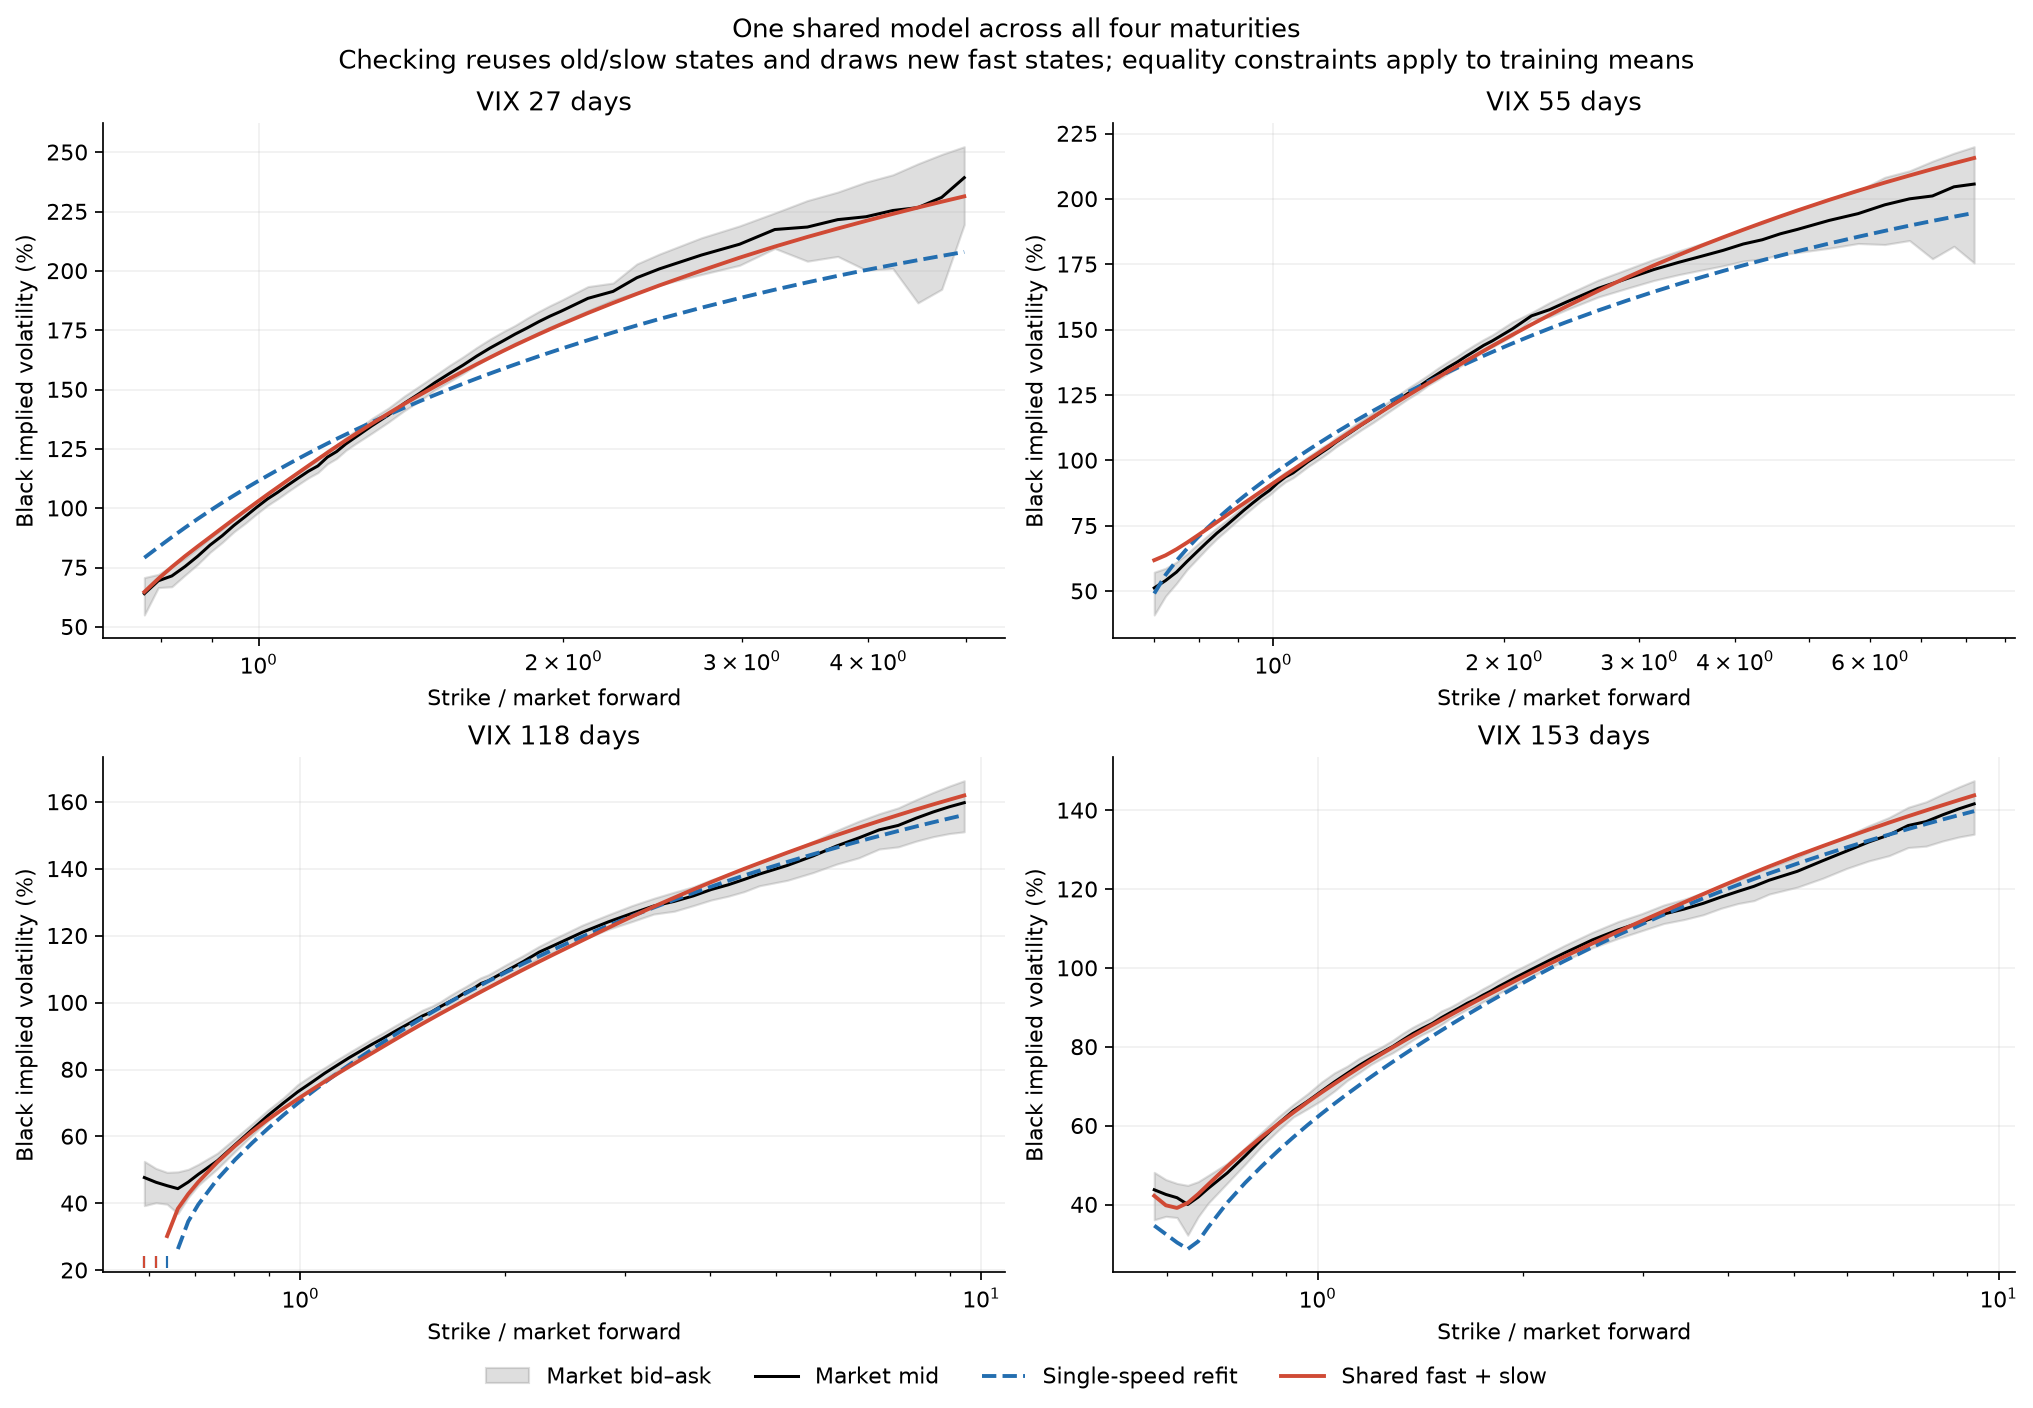
\includegraphics[width=\linewidth,height=.78\textheight,keepaspectratio]{figures/vix-two-speed-smiles.png}
\caption{Archived all-maturity VIX comparison from the two-speed study. Both speeds and all mixture parameters are shared. The source plot's IV convention and sampling bands apply; bands are not bounds on total numerical error. Source: R13.}
\end{figure}

\subsection{Four fixed stress speeds}
Four shared half-lives, 7/28/112/448 days, were fixed before fitting. Checking option loss was 0.06216 versus 0.05008 for two speeds; paired increase 0.01208 had SE 0.02412. Forward checking error reached about 0.216 points despite near-exact training equalities. \src{R14b}

This is neither an improvement nor a resolved superiority comparison. The geometric grid is not a nested extension of the fitted two-speed model, so the result does not establish that four factors are intrinsically worse. No SPX work was done in that test.

\section{Why the good VIX model did not automatically fit SPX}
\subsection{The first two-speed joint refit}
The joint trial freed 16 curve levels, the floor and six stress parameters, while keeping original M2 coefficients fixed. The two stages were iteration-limited local searches. \src{R15}

\begin{center}\begin{tabular}{lrr}\toprule
Checking quantity & VIX-only parameters & Joint parameters\\\midrule
SPX interval loss & 5467.10 & 618.74\\
VIX option loss & 0.05008 & 37.9711\\
SPX inside bid--ask & 9/1294 & 9/1294\\
VIX inside bid--ask & 153/217 & 20/217\\
Stress weight $w$ & 0.92284 & 0.01943\\\bottomrule
\end{tabular}\end{center}
The joint fit nearly removes stress, deactivates the slow branch and moves the floor to 5\%. Its SPX checking estimates include 20 negative values. It finds a sampled compromise, not simultaneous calibration.

One structural interpretation is that independent stress supplies variance dispersion without directly associating stress shocks with equity declines. At high stress weight, the variance mechanism already correlated with equity has a small mean allocation. This motivates adding negative stock--stress dependence. It is an interpretation supported by the later leverage response, not proof that independence was the sole cause.

\subsection{Protecting VIX and changing only off-window variance}
VIX contracts see seven of the 16 curve levels; the other nine lie outside the union of their four averaging windows. Changing those nine leaves the full VIX law unchanged in the exogenous model, while changing integrated stock variance. This is a genuine separation of identifiable inputs, not a claim that VIX identifies the whole curve. \src{R16b}

The protected curve fit improved fresh SPX price loss 5979.32 to 3895.07, but IV MAE worsened 4.345 to 4.710 pp and inside-bid--ask count fell 11 to 8. It corrected price levels without repairing the required downward skew. Its VIX preservation is inherited mathematical invariance, not a fresh proof that existing numerical forward errors vanished.

\lesson{Variance scheduling and equity skew are different controls. Curve-only fitting can improve a price score while making the displayed IV fit worse. Repeating that same search does not address the missing dependence mechanism.}

\section{Correlating equity and stress shocks}
\subsection{A rotation that changes SPX but preserves VIX}
With $W^0$ the old stock Brownian motion and independent stress drivers $B^s,B^f$, define
\begin{equation}\label{eq:rotation}
dW_t^{S,\theta}=\sqrt{1-\theta^2}\,dW_t^0
-\theta(c_s\,dB_t^s+c_f\,dB_t^f),\quad c_s^2+c_f^2=1.
\end{equation}
Its variance is $dt$. Positive stress shocks now tend to lower stock while raising variance. The factor dynamics, their joint law and readout remain fixed, so the VIX law is unchanged. Independence here is between stress and old drivers; $W^0$ already has its old-bank dependence. Those old stock--M2 correlations shrink by $\sqrt{1-\theta^2}$. \src{R17}

In general, if $dv_t=\cdots+\mathbf k_t\cdot d\mathbf B_t$ and stock has unit exposure $\mathbf a_t$, then
\begin{equation}
d\langle\log S,v\rangle_t=\sqrt{v_t}\,\mathbf a_t\cdot\mathbf k_t\,dt.
\end{equation}
More negative covariance associates falling equity with rising variance, a useful downside-skew mechanism. It does not guarantee a particular option slope.

The scan tested $\theta=0,.2,.4,.6,.8,.95$, with mixed, fast-only and slow-only directions. Mixed used $(c_s,c_f)=(\sqrt{1-r},\sqrt r)$. Mixed $\theta=.8$ was selected before new expensive checking. Price loss fell 3788.48 to 1861.38 and IV MAE 4.493 to 3.199 pp. The approximate paired loss-change interval excluded zero, but omitted deterministic bias. Only 18/1294 prices were inside bid--ask; median SE was 1.36 quote scales.

At 29 days, IV(right)$-$IV(left) near $K/F=.9,1.1$ moved from $-1.52$ to $-5.58$ pp; market was $-14.05$ pp. It moved in the right direction, but not far enough. Mixed exposure beat the isolated directions in the reported comparison. $\theta=.95$ looked slightly better on checking, but was not the preselected winner and is not a uniquely validated optimum.

\textbf{What is special about this experiment?} It changes stock's coupling to a fixed factor system. Arbitrarily changing correlations \emph{between variance-factor drivers} can change the VIX law. Endogenous return feedback can change it too. VIX invariance is specific to the construction, not a universal fact about adding correlation.

\begin{figure}[!htbp]
\centering
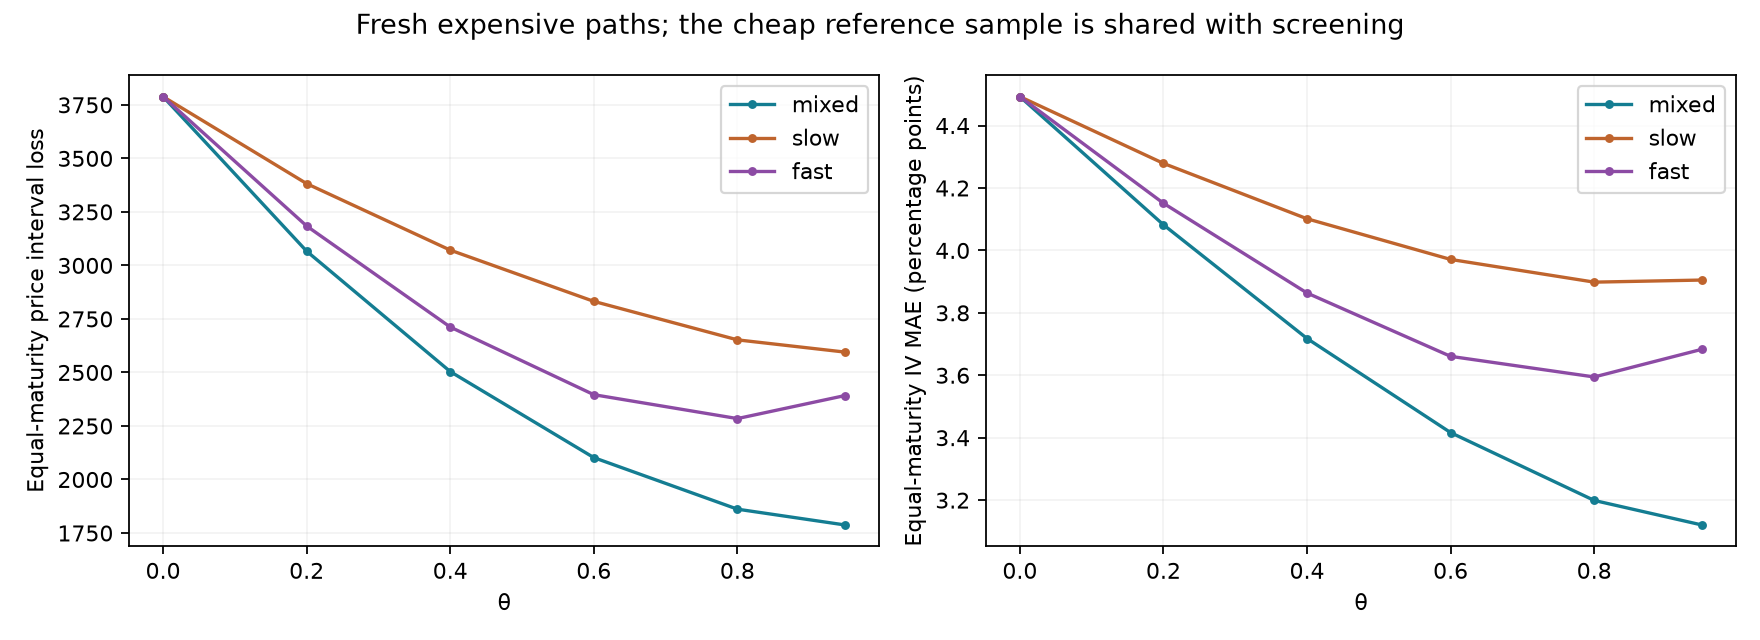
\includegraphics[width=\linewidth,height=.77\textheight,keepaspectratio]{figures/SPX-response.png}
\caption{Archived response to constant stock--stress rotation. This comparison changes stock dependence while retaining the successful variance-factor/VIX law. It is a partial SPX improvement, not a satisfactory calibration. Source: R17.}
\end{figure}
\clearpage

\subsection{Adaptive loading opposite instantaneous variance sensitivity}
For a given $\mathbf k_t$, the most negative instantaneous covariance among unit stock directions is obtained by
\begin{equation}
\mathbf a_t=-\mathbf k_t/\|\mathbf k_t\|.
\end{equation}
This follows from Cauchy--Schwarz. The implemented construction uses all relevant old-bank and stress directions with a declared zero-gradient convention. The factors and VIX law stay fixed. \src{R21}

On the finer paired check, SPX loss changed 1869.58 to 1821.00 and IV MAE 3.203 to 3.040 pp, but four IVs became invalid and approximate paired loss-change intervals included zero. The 29-day gap was $-4.90$ pp versus baseline $-5.22$ and market $-14.05$. Maximizing instantaneous negative covariance did not maximize the needed finite-maturity skew.

\subsection{Loading opposite future integrated-variance sensitivity}
The next rule targeted persistence directly. Define, for the same 30-day lookahead everywhere,
\begin{equation}
J(t,\mathbf X_t)=\E\!\left[\int_t^{t+30/365}v_u\,du\,\middle|\,\mathcal F_t\right],
\qquad dJ_t=\cdots+\mathbf K_t\cdot d\mathbf B_t.
\end{equation}
Use stock direction $-\mathbf K_t/\|\mathbf K_t\|$, updated four or eight times per trading day. This uses conditional expectations, not realized future information. The complete state and individual OU decay speeds enter the sensitivity. VIX remains unchanged. \src{R22}

At 256 stock steps/day, fixed-direction SPX loss was 1909.19 and the eight-update future rule gave 1941.31, a 1.68\% increase. IV MAE changed 3.201 to 3.157 pp; the 29-day gap became less negative, $-6.39$ to $-4.51$ pp. All approximate paired loss-change intervals included zero. This particular horizon and direction rule did not demonstrate improvement. It does not rule out every state-dependent correlation.

\lesson{Negative constant stress leverage was a substantial useful change. The tested attempts to optimize the stock direction locally or over a 30-day future-variance signal did not close the remaining SPX gap. The next distinct question concerns the readout's memory, rather than another repeat of the same correlation scan.}

\section{Asymmetric readouts after the successful VIX fit}
\subsection{Multiplying the whole response by bad-news sensitivity}
Keeping the mixed rotation at $\theta=.8$, we used the existing standardized feedback factor $X_t$ and
\begin{equation}
D_\alpha(X)=e^{\alpha\splus(-X)},\qquad
H_t^\alpha=\frac{H_t^0D_\alpha(X_t)}{\E[H_t^0D_\alpha(X_t)]}.
\end{equation}
It raises raw variance in negative-feedback states. All original readout/stress coefficients were fixed; seven VIX-window curve levels were refitted under four training forward equalities. \src{R26}

At $\alpha=1.5$, fresh SPX available-IV MAE improved 3.278 to 2.832 pp, but VIX loss rose about 0.047 to 25.725; six SPX IVs were invalid and stock SEs increased. No positive tested strength passed the declared VIX-preservation screen, so the selection retained $\alpha=0$.

Why did nominally fixed stress weight fail to protect VIX? Let $H^0=(1-w)R+wA$, with $\E[A]=1$ and $A$ independent of the old bank. Then
\begin{equation}
\E[H^0D]=(1-w)\E[RD]+w\E[D].
\end{equation}
The mean stress share after normalization is
\begin{equation}
\frac{w\E[D]}{(1-w)\E[RD]+w\E[D]},
\end{equation}
which need not equal $w$. At 153 days it fell from 92.3\% to 53.2\% at $\alpha=1.5$. The stronger downside readout also reallocates mean variance away from the successful stress mechanism.

A four-way ablation is especially instructive:
\begin{center}\begin{tabular}{lrr}\toprule
Variant & 29-day IV(right)$-$IV(left) & VIX loss\\\midrule
Original & $-5.86$ pp & 0.050\\
Multiplier only & $-6.05$ pp & 21.278\\
Curve only & $-8.51$ pp & 19.400\\
Both & $-13.44$ pp & 25.725\\
Market gap & $-14.05$ pp & \\\bottomrule
\end{tabular}\end{center}
The striking combined short-expiry skew cannot be credited to the multiplier alone. The first changed VIX-window curve interval also spans days 27--29, affecting 29-day SPX. The interaction is nonlinear, and other maturities remain mismatched.

\subsection{Normalizing separately within each stress state}
The subsequent regime construction was
\begin{equation}
H^{\rm reg}=H^0D\frac{a+wA}{a\E[RD]+wA\E[D]},\qquad a=1-w.
\end{equation}
By independence,
\begin{equation}
\E[H^{\rm reg}\mid Z^s,Z^f]=a+wA,\qquad \E[H^{\rm reg}]=1.
\end{equation}
It preserves the mean response \emph{within each current stress state}, more than global normalization does. It does not preserve the internal branch budgets separately or the whole conditional future variance law. Consequently it does not preserve VIX. \src{R21}

At strength 1.5 with seven-level refit, VIX loss was 6.159 rather than 25.725 for the global multiplier on the same VIX checking streams. This is less damage, but far worse than the baseline near 0.050. Finer-check SPX loss was 1560.53 and IV MAE 2.897 pp against baseline 1869.58 / 3.203 pp; two IVs were invalid and paired loss intervals included zero. The 29-day gap was only $-6.29$ pp. No positive strength passed the VIX-preservation screen.

\lesson{Mean-one normalization, conditional mean preservation and full VIX-law preservation are different guarantees. The experiments explicitly demonstrate the gap between them.}

\section{Numerical changes: what they taught us without changing the model}\label{sec:numerics}
Many weeks of work concerned how accurately we price a fixed model. These experiments should not be interpreted as economic model modifications. \src{R01,R27}

\subsection{Rare tails and conditional VIX integration}
Direct Gaussian second-moment checks agreed with the target more closely than early outer simulations. Refining selected conditional quadrature/normalizer states did not explain the discrepancy. Rare outer paths were the leading explanation; no universal normalizer bug or complete convergence result was established.

Defensive importance sampling removed zero-hit cases at tested budgets. Learned pilots and stratified allocations improved some option errors but often worsened forwards. Score-covariance inflation generally lost. Known-mean Gaussian controls helped forwards, but most option screens still failed. Matching $\E[\VIX^2]$ did not imply accurate wing calls or $\E[\VIX]$.

\subsection{SPX importance sampling, controls and conditioning}
Equity-path tilts and volatility-excursion proposals increased tail exposure. The vol7/ridge5 control estimator became a working historical reference, not a universal optimum. Stronger upward call tilts increased hits without broad efficiency gains.

MLMC on 64/128/256/512 grids lost the measured central variance--cost comparison. Endpoint-preserving bridge reflection also lost. Nine OU innovation controls gave variance gains largely consumed by runtime; three linear controls gave modest representative efficiency but failed broader stability/positivity checks. In a 24-contract central panel, no primary sampling screens passed.

Partial conditional Monte Carlo integrated an independent equity direction. That direction represented only 0.6367\% of equity Brownian variance in the old architecture. Raw conditional variance gain was modest; conditioning existing controls plus a retained-path proposal lost whole-panel variance--cost. Small independent Brownian variance is not a theorem bounding all possible conditioning gains.

For the independent-stress two-speed model, a cheap stress-only auxiliary stock, paired full-M2 correction and exact discrete conditional martingale correction improved median SEs roughly 8--29 fold. Yet only 1/1294 primary quotes passed the screen in that phase; the expensive full-M2 correction remained the bottleneck. Subsequent bounded fitting was explicitly exploratory. \src{R16b}

\subsection{Parity and continuous controls changed the comparison convention}
Discount-suppressed parity gives
\begin{equation}
C-P=F-K.
\end{equation}
Market puts convert to canonical calls using the market forward. Model puts use the \emph{model} forward. For VIX,
\begin{equation}
e_{\rm canonical\ call}=e_{\rm native\ put}+F_{\rm model}-F_{\rm market}.
\end{equation}
Thus common-call and native-OTM objectives differ when the VIX forward is wrong. Converting representation does not repair the forward. One final scheme used the same call construction and all 4096 paths at every strike; earlier adaptive-prefix allocation was superseded. \src{R09}

Continuous interpolation of \emph{zero-mean control draws} removed nearest-donor switching. This is not smoothing the price or IV curve. A natural-cubic variant worsened shape flags and was rejected. Signed controls can still yield negative estimates or sample convexity failures; raw positive payoffs can still miss rare events.

\subsection{The four accuracy questions we must keep separate}
\begin{enumerate}
\item \textbf{Sampling error:} variation across genuinely independent batches, with antithetic pairs and shared references handled correctly.
\item \textbf{Stock-grid error:} exact OU transitions do not make nonlinear log-stock integration exact. Even 512 steps/day is not automatic convergence.
\item \textbf{Normalizer error:} Gaussian quadrature and time interpolation require their own checks.
\item \textbf{Conditional VIX error:} full-state conditional expectations and integration over the 30-day window introduce different approximations.
\end{enumerate}
The established sampling screen was $2\,\mathrm{SE}\leq s_i/4$, equivalently $\mathrm{SE}\leq s_i/8$. Bias is separate. A zero empirical SE with no payoff hits is not a pass. A finite ensemble can satisfy training forward constraints almost exactly while fresh checking misses the forward materially.

No negative estimate was converted into an acceptable quote by clipping. Missing IVs remain missing. Available-IV MAE must be read alongside their counts. Old validation streams, reused reference prices and the single market snapshot prevent claims of untouched market validation.

\section{A compact map of tested changes}
\small
\begin{longtable}{@{}>{\raggedright\arraybackslash}p{.22\linewidth}>{\raggedright\arraybackslash}p{.25\linewidth}>{\raggedright\arraybackslash}p{.25\linewidth}>{\raggedright\arraybackslash}p{.20\linewidth}@{}}
\toprule Change & SPX consequence & VIX consequence & Assessment\\\midrule\endhead
Slower spike lift; shifted feedback & Synthetic leverage/tails/Zumbach balance improves & Not an option-fit test & Useful P baseline, R02\\
Orthogonal energy; echo & Small P roughness gain; echo negligible & Not jointly calibrated & Optional O; echo off, R02\\
Fine-grid P refit & Leverage improves; rank Zumbach fails validation & No Q option fitting & Coarse success qualified, R28\\
Positive spike shift & Stronger downside asymmetry; P gates can deteriorate & Later Q fits retain positive shift & Joint tradeoff, R03\\
State plus curve refit & Better pooled sampled score & Mixed expiry effects & State and curve confounded, R04\\
Three to five curve pieces & Small inconsistent extra gain & No smile-shape solution & Not adopted, R04\\
Sixteen aligned pieces & Moderate training gain & Budget/price gain; flat wings remain & Useful flexible curve, R06\\
Original readout refit & Controlled trial improves aggregate SPX & Aggregate improvement; long-date costs & Provisional, R07--09\\
Cap variants & Cleaner selections worsen SPX & Better wings, worse ATM / uncertain total gain & No joint remedy, R12\\
Cluster-weighted spike mixture & Not fully priced & Tested VIX profiles worsen & No immediate remedy, R12\\
Spike sensitivity dial & Selected full SPX cases much worse & Wing levels closer, slopes flatter & Fixed-curve failure, R14\\
After-cap multiplier & Strong case worse; mild gain uncertain & Strong shape gain, no price-fit gain & No adoption, R16\\
Seven active curve levels & Not priced in VIX-only trial & Budget improvement, weak shape gain & Necessary, insufficient, R11\\
Product response mixture & Not priced in that trial & Modest gain & Less effective than additive, R18\\
Additive M2/stress & Not priced in that trial & Large shape gain; short slopes overshoot & Stress dominates, R18\\
Tight forwards; free floor & Not priced in that trial & Strong improvement; floor at bound & Partial VIX result, R19\\
Continuous Beta measure & Not priced in that trial & No gain over endpoint mixture & Complexity unnecessary here, R20\\
Shared two speeds & Later frozen model has poor SPX skew & Large option-fit gain across four dates & Best partial VIX evidence, R13\\
Four geometric speeds & Not priced & No demonstrated gain; forward gaps & No automatic benefit, R14b\\
Joint two-speed refit & Large sampled price gain; poor accuracy & Successful smile largely lost & Stress almost removed, R15\\
Protected off-window curve & Price loss down, IV error up & Entire law preserved & Level change insufficient, R16b\\
Constant stress rotation & Material price and IV improvement & Entire law preserved & Promising, still poor fit, R17\\
Adaptive instantaneous direction & Small uncertain aggregate change & Entire law preserved & Local covariance insufficient, R21\\
Future-variance direction & No demonstrated improvement & Entire law preserved & One 30-day rule tested, R22\\
Whole-response asymmetry & Some IV gain; strong grid/tail costs & Severe deterioration & Mean stress share changes, R26\\
Stress-regime normalization & Modest uncertain gains & Less damage, still poor & Conditional mean insufficient, R21\\
Sampling/control refinements & Sometimes large precision gains & Sometimes large precision gains & Accuracy, not new economics, R27\\\bottomrule
\end{longtable}
\normalsize

\section{What remains open, and what we should retain}
\subsection{A coherent interpretation of the tradeoff}
Our evidence supports the following working picture. Flexible average variance helps maturity levels and can remove a hard moment-budget obstruction. Additive stress and multiple persistence scales help VIX shape. Correlating stock with those same stresses restores some equity downside skew. However, the current response and memory do not produce enough short-expiry SPX skew while preserving the successful VIX smiles. Stronger whole-response asymmetry changes the variance allocation and disrupts VIX.

This picture is narrower than a theorem. We have not performed a fully accurate global optimization of all readout, curve, stress and dependence parameters, nor established impossibility for the family. Several promising comparisons remain noisy, bounded or iteration-limited.

\subsection{A distinct next hypothesis: memory in the existing readout}
The latest stationary Gaussian diagnostic of feedback $Y$ gives autocorrelations about 0.170 after one day, 0.048 after seven days and 0.017 after 30 days. This is a model-memory calculation, not a historical estimate or proof of the cause of SPX misfit. Slower OU modes already exist. \src{R22}

Giving a slower projection a separate asymmetric role, while preserving the fast Zumbach-motivated component, is a concrete new hypothesis. It could change how long bad-news states influence variance. It remains \emph{untested}: it requires a new readout, normalizers, stock prices and conditional VIX calculations. No new bank or slower readout has been adopted.

Other previously discussed ideas must also remain correctly labeled. Broad Q-risk-price comparisons were proposed but deferred in the documented pricing sequence; existing synthetic structural scenarios do not constitute a completed option-fit comparison. A new Gamma-driven bank, a new continuous stochastic noise-amplitude process, arbitrary continuous speed measures, quintic readouts and jump-based remedies are not completed M2 joint-calibration results.

\subsection{How to interpret Othmane's later architecture}
The October external specification is different from checked-in A2. It includes noise-amplitude modulation and an equity-feedback bank, schematically
\begin{equation}
ds_t^j=-\kappa_js_t^jdt+\sqrt{2\kappa_j}\,
\frac{\sigma_t}{\widetilde\sigma(t)}\,dW_t^X.
\end{equation}
Changing the readout then changes future $s$ paths. Our M2 readout layers leave the original OU law exogenous. The external Gamma process modulates \emph{bank noise}; our added exponential and spike-dial factors modify the \emph{readout}. These are not equivalent constructions. Its noise modulation can be written $dr_i=-\lambda_i r_i\,dt+\sqrt{2\lambda_i\Gamma_t}\,dW_i$, with positive jump-driven $\Gamma$. The reported Gamma jump modulation is not a direct stock-price jump model. \src{R10,R24}

The later report's bounded flexible readout is
\begin{equation}
\sigma_t=\widetilde\sigma(t)e^{\psi(\zeta_t)}F(P_t),\qquad
\widetilde\sigma(t)=a e^{-bt}+c(1-e^{-bt}).
\end{equation}
Here $\psi$ is a decreasing piecewise-linear log-volatility response, flat beyond $\pm3$, with five pieces and $\psi(0)=0$. The feedback multiplier $F(P)$ has four loss-side pieces and one gain-side piece, $F(0)=1$, and flat outer tails. This directly separates asymmetric loss/gain responses from the rough-bank response. Its time curve is a volatility scale, not our explicitly normalized expected-variance curve $\xi$. These are externally reported readouts; they were not substituted into M2 in a completed common-protocol trial. \src{R24}

The later external option report retains VIX-wing and approximate-estimator limitations; there is no source-matched common-protocol repricing establishing that architecture as a solved double calibration. Its endogenous feedback is outside the currently preserved exogenous-only design. This is context, not an additional M2 experiment or a certified model ranking.

\subsection{What is reusable, and what is actually proved}
For fixed exogenous dynamics, readout changes reuse OU paths and common random draws, \emph{not} old variance or stock prices. Initial-state shifts have the form $e^{-\Lambda t}\Delta X_0$, but downstream quantities still change. Altered OU rates require a new state construction; endogenous feedback generally requires resimulation.

For fixed variance paths the rotation has an especially cheap reconstruction:
\begin{equation}
\log(S_T/S_0)=-\tfrac12 I+\sqrt{1-\theta^2}U_0-\theta(c_sU_s+c_fU_f),
\end{equation}
where $I=\sum v\,dt$ and $U_i=\sum\sqrt v\,\Delta B^i$. Readout/curve changes require rebuilding these sums. Adaptive exposures cannot in general reuse this same fixed finite set.

Existing Lean work proves scoped algebraic facts, including response curvature, a moment-payoff inequality, rotation coefficient normalization and an abstract discrete reconstruction. Exact-rational quote certificates address archived finite data. Numerical derivative, covariance and replay checks address implemented calculations. These are different forms of evidence. They are not a formal proof of the full simulator, continuous stock martingality, population VIX-forward equality or calibration convergence. No new Lean audit was run for this report.

The durable assets are the interpretable mean-one variance framework, the budget feasibility test, the strong two-speed VIX candidate, the VIX-preserving leverage construction, and the preserved unsuccessful experiments. Together they tell us which changes moved levels, which changed shape, which merely improved precision, and which questions remain genuinely new.

\appendix
\section{Evidence register and reproduction context}
This report was checked against the current local result notes, their linked model equations and the latest research ledger. Numerical tables reproduce recorded results; simulations and optimizers were not rerun. The record is not a certified meta-analysis of every archived array. Some older run trees are absent or changed in the working checkout, so the source notes and their stated audits remain the evidence for historical numbers.

Current primary SPX counts are 277, 298, 228, 141, 167, 112 and 71 at the seven dates in ascending order, totaling 1294 of 1751 eligible quotes. VIX counts are 49, 58, 55 and 55 at the four dates in ascending order, totaling 217. Current feasibility work has no market holdout. Earlier 707-SPX/175-VIX results retain their historical scope.

Unless a different directory is given below, paths are relative to
\begin{center}\small\path{matteo/model_comparison/option_pricing/}\end{center}
Each note links its run directory, original sources, parameters, numerical setup and limitations. These local paths are intentionally included so the report remains auditable from the repository.
\footnotesize
\setlength{\parskip}{3pt}
\begin{description}[style=nextline,leftmargin=1.5em,labelindent=0pt,itemsep=0pt,parsep=0pt]
\item[R01] \path{RESEARCH_LEDGER.md}; \path{active_scope.json}. Latest chronology and retained scope.
\item[R02] \path{matteo/exogenous_reservoir_eq_m2/experiments/EXPERIMENT_COMPARISON.md}; original M2 specification in \path{matteo/exogenous_reservoir_eq_m2/documentation/esn_exponential_quadratic_model.tex}. Paths from repository root.
\item[R03] \path{matteo/exogenous_reservoir_eq_m2/experiments/asymmetry_001/RESULTS.md}, from repository root.
\item[R04] \path{JOINT_STATE_REFINEMENT_RESULTS.md}. Restricted states and nested five-piece curve.
\item[R05] \path{ALL_MATURITY_FIT_RESULTS.md}. Expanded in-sample scope.
\item[R06] \path{MATURITY_CURVE_FIT_RESULTS.md}. Sixteen-piece maturity-aligned curve.
\item[R07] \path{FULL_READOUT_FIT_RESULTS.md}. Raw-payoff eleven-parameter trial.
\item[R08] \path{CONTROLLED_READOUT_EXPLORATION_RESULTS.md}. Restored-precision controlled trial.
\item[R09] \path{PARITY_UNIFORM_RESULTS.md}; \path{PARITY_ADAPTIVE_RESULTS.md}; \path{PARITY_PARAMETER_FIT_RESULTS.md}; \path{JOINT_LOCAL_ACCELERATION_RESULTS.md}. Parity, controls and subsequent local fits.
\item[R10] \path{STOCHASTIC_VOL_OF_VOL_RESEARCH.md}; \path{WING_MECHANISM_FINDINGS.md}. Quote-budget certificates, illustrative marginal mechanism and external-model distinctions.
\item[R11] \path{VIX_ONLY_CURVE_RESULTS.md}. Seven active curve levels.
\item[R12] \path{CAP_TAIL_RESULTS.md}; \path{CAP_TAIL_MATHEMATICS.md}; \path{CAP_CONTROLLED_RESULTS.md}. Cap families, moment domain and cleaner comparison.
\item[R13] \path{TWO_SPEED_RESULTS.md}; \path{TWO_SPEED_PLAN.md}. Shared fast/slow model, parameters and four-expiry outcomes.
\item[R14] \path{STOCHASTIC_VOV_RESULTS.md}. Inside-score spike-sensitivity dial.
\item[R14b] \path{STRESS_BANK_RESULTS.md}. Fixed geometric four-speed comparison.
\item[R15] \path{TWO_SPEED_JOINT_RESULTS.md}. Restricted 23-parameter joint refit.
\item[R16] \path{POSTCAP_VOV_RESULTS.md}. Independent after-cap amplitude.
\item[R16b] \path{TWO_SPEED_PRECISION_RESULTS.md}; \path{PROTECTED_CURVE_RESULTS.md}; \path{PROTECTED_CURVE_CONCLUSION.md}. Protected VIX and off-window fitting.
\item[R17] \path{LEVERAGE_SCAN_RESULTS.md}; \path{SPX_SKEW_RESEARCH_AND_FAST_ABLATIONS.md}. Constant negative stress rotation and scoped formal bridge.
\item[R18] \path{MIXED_RESPONSE_RESULTS.md}. Product and additive response trials.
\item[R19] \path{FORWARD_FLOOR_RESULTS.md}. Forward equalities and free floor.
\item[R20] \path{CONTINUUM_RESPONSE_RESULTS.md}; \path{CONTINUUM_INITIAL_RESULTS.md}. Continuous Beta measure and estimator repair.
\item[R21] \path{TARGETED_SKEW_RESULTS.md}. Instantaneous gradient loading and conditional stress normalization.
\item[R22] \path{FORWARD_LEVERAGE_RESULTS.md}. Future-variance loading and readout-memory diagnostic.
\item[R23] \path{JOINT_CURVE_FIT_RESULTS.md}; \path{CALIBRATION_PROGRESS.md}. Early joint tradeoff and objective definitions.
\item[R24] \path{SimultanuousAllFeatures/joint_calibration_protocol.tex}, from repository root; external October architecture discussion in R10 and \path{matteo/model_comparison/othmane_docs_20261026.prepared/cs_doc/original.pdf}, p.3 (readout equations visually checked), from repository root. The legacy protocol describes its own conventions and is not a source-matched joint-option result.
\item[R25] \path{matteo/model_comparison/othmane_replication/RESULTS.md}, from repository root. Historical nine-asset comparison and early readout screen.
\item[R26] \path{ASYMMETRIC_READOUT_RESULTS.md}. Global bad-news multiplier and four-way ablation.
\item[R27] Numerical studies grouped in the ledger, including \path{VIX_MOMENT_DIAGNOSIS.md}, \path{VIX_IMPORTANCE_SAMPLING_RESULTS.md}, \path{VIX_GAUSSIAN_STABILITY_RESULTS.md}, \path{SPX_MLMC_RESULTS.md}, \path{SPX_BRIDGE_COUPLING_RESULTS.md}, \path{SPX_CENTRAL_PANEL_RESULTS.md}, \path{SPX_CONDITIONAL_PRICING_RESULTS.md} and \path{SPX_CONDITIONAL_CONTROL_RESULTS.md}. Their scope and conclusions are summarized in Section~\ref{sec:numerics}; this report does not rerun their accuracy audits.
\item[R28] Physical follow-ups from repository root: \path{matteo/exogenous_reservoir_eq_m2/experiments/timestep_convergence_001/RESULTS.md}; \path{matteo/exogenous_reservoir_eq_m2/experiments/stage4_fine_grid_001/RESULTS.md}; \path{matteo/exogenous_reservoir_eq_m2/experiments/zumbach_discrepancy_001/RESULTS.md}; \path{matteo/exogenous_reservoir_eq_m2/experiments/pearson_zumbach_001/README.md}; \path{matteo/exogenous_reservoir_eq_m2/experiments/physical_stability_001/RESULTS.md}.
\end{description}
\normalsize
\end{document}
